\newcolumn
\section{Leitungsmodell}

\subsection{Leitungsgleichungen}
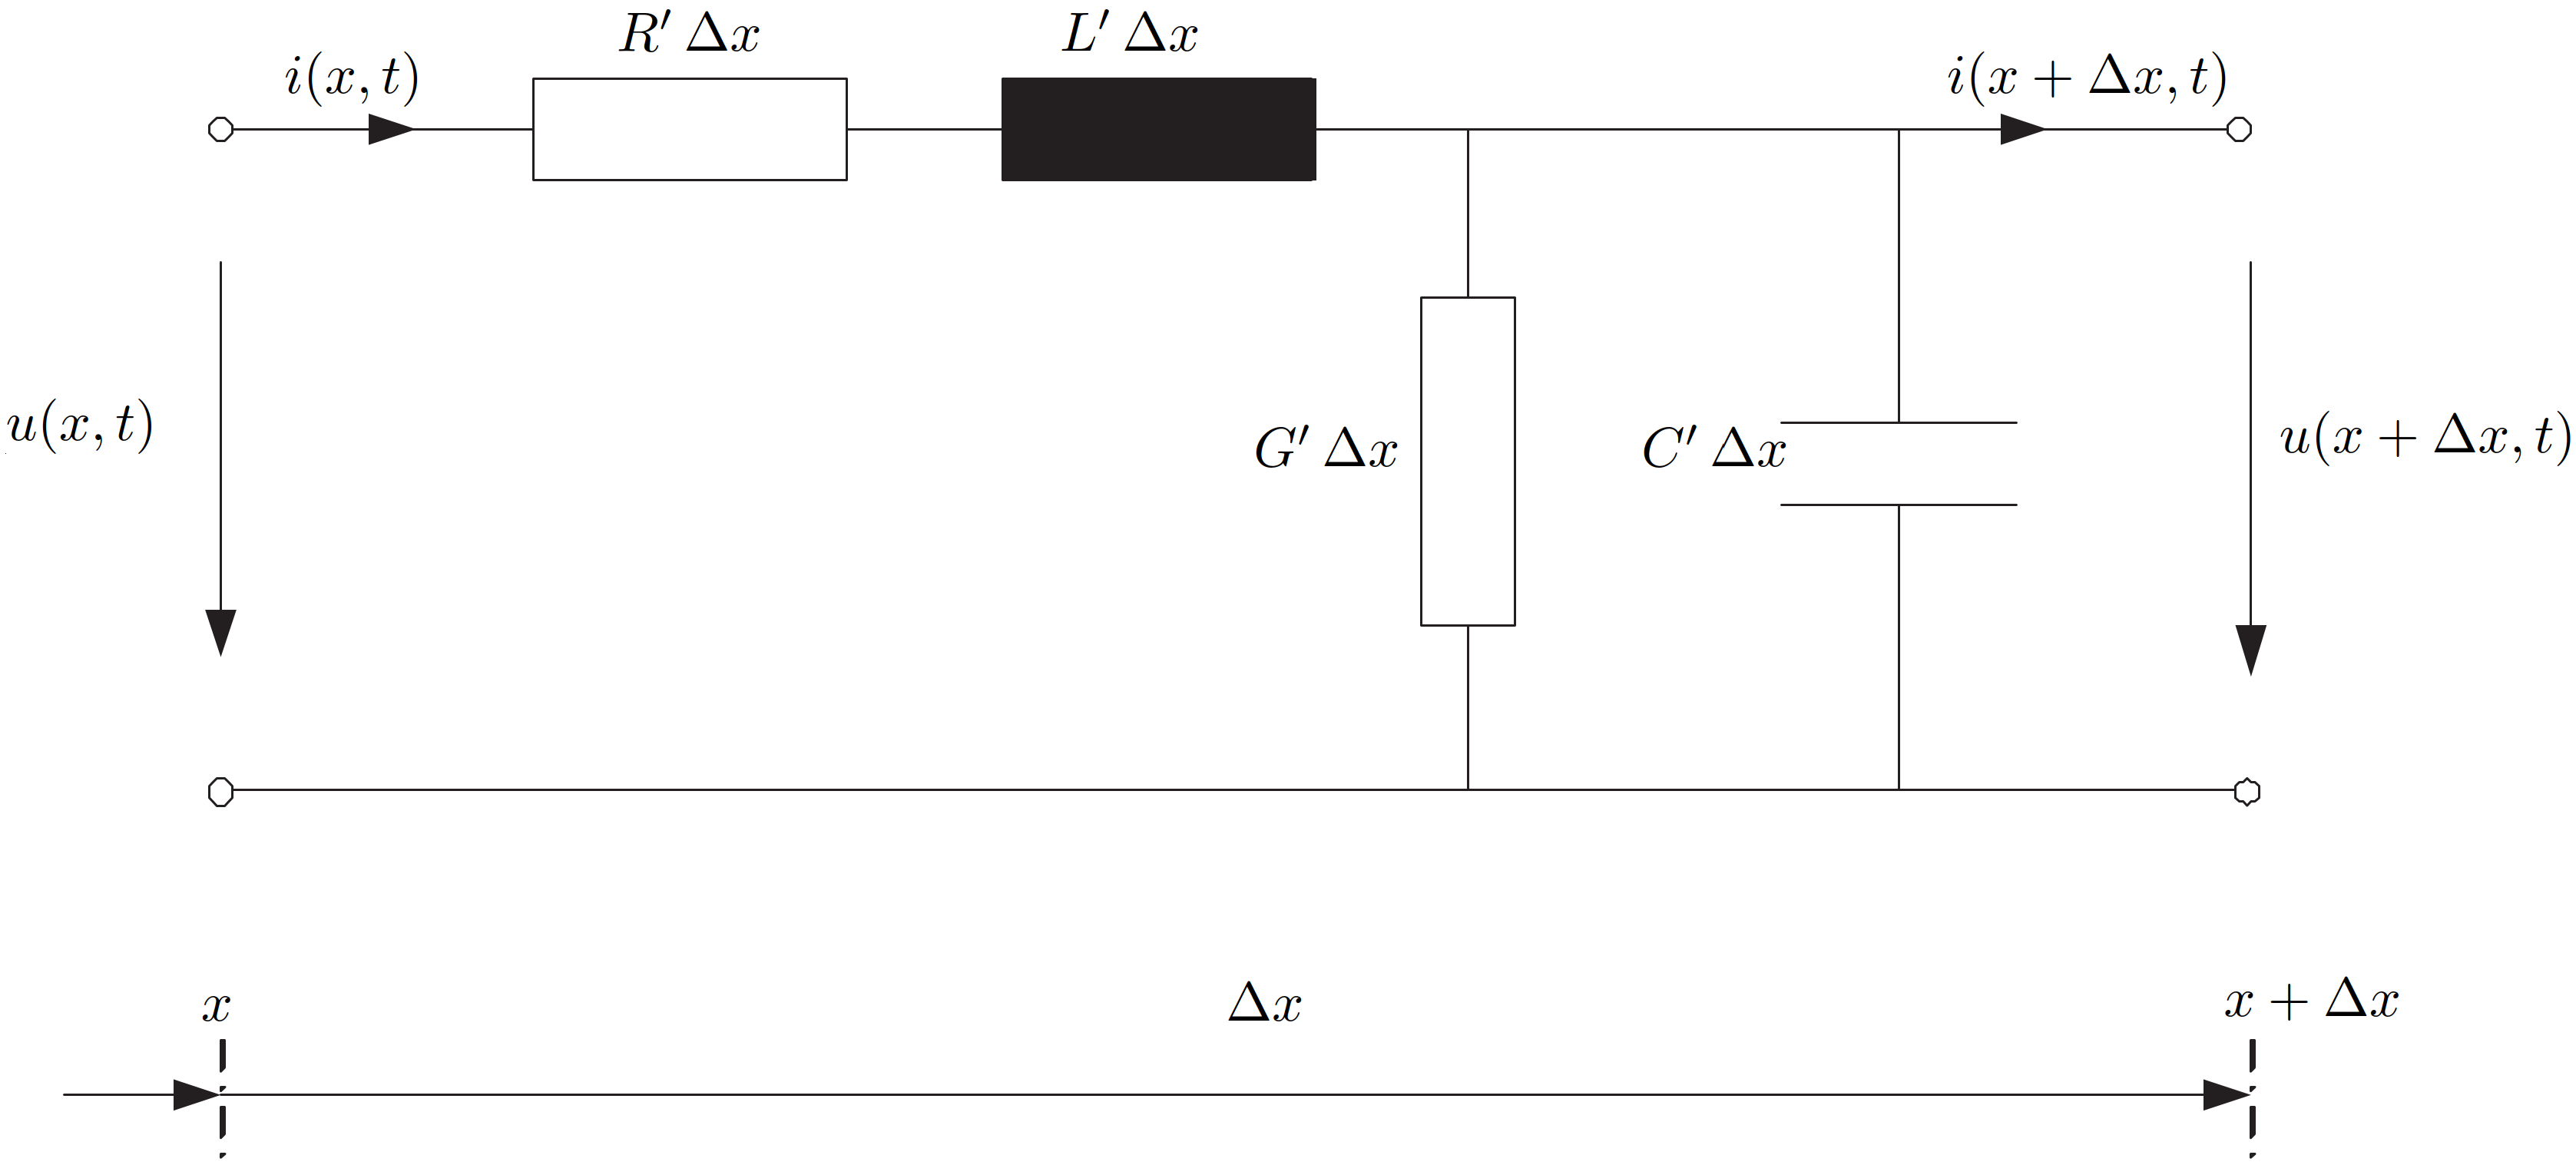
\includegraphics[width=0.98\columnwidth, align=c]{images/Leitungsgleichungen_1.png}

\subsubsection{Allgemeine Differential Gleichung}
 
    \vspace{0.15cm}
    $
    \boxed{\frac{\partial u}{\partial x} = -\left(R' + L' \frac{\partial}{\partial t}\right)  \cdot i}
    \quad
    \boxed{\frac{\partial i}{\partial x} = -\left(G' + C' \frac{\partial}{\partial t}\right)  \cdot u}
    $
    \vspace{0.15cm}

\subsubsection{Allgemeine Differential Gleichung für Wechselstrom}
    
    \vspace{0.15cm}
    $
    \boxed{\frac{\partial U}{\partial x} = -\left(R' \cdot I + j \omega L' \cdot I\right)}
    \quad
    \boxed{\frac{\partial I}{\partial x} = -\left(G' \cdot U + j \omega C' \cdot U\right)}
    $

\subsubsection{Weitere Gleichungen}

$
\boxed{\frac{d^2 U}{dx^2} = \left(R' + j \omega L'\right)\left(G' + j \omega C'\right) \cdot U}
$

$
\boxed{\frac{d^2 I}{dx^2} = \left(R' + j \omega L'\right)\left(G' + j \omega  C'\right) \cdot I}
$

\vspace{0.15cm}

Mit folgender Definition von $\gamma$ ergibt sich:

\vspace{0.15cm}

$
\boxed{\underline{\gamma} = \sqrt{(R' + j\omega L')(G' + j \omega C')} = \alpha + j\beta}
$

$
\boxed{\frac{d^2 U}{dx^2} = \underline{\gamma}^2 \cdot U}
$

$
\boxed{\frac{d^2 I}{dx^2} = \underline{\gamma}^2 \cdot I}
$


\subsection{Lösung der Leitungsgleichung}

$
\boxed{\underline{U}(x) = \underline{U}_a + \underline{U}_b = \underline{U}^+ \cdot e^{-\underline{\gamma} x} + \underline{U}^- \cdot e^{\underline{\gamma} x}}
$

$
\boxed{\underline{I}(x) = \underline{I}_a + \underline{I}_b = \underline{I}^+ \cdot e^{-\underline{\gamma} x} + \underline{I}^- \cdot e^{\underline{\gamma} x}}
$

$
\boxed{\underline{I}(x) = \frac{-1}{R' + j\omega L'} \cdot \frac{d\underline{U}}{dx}
= \sqrt{\frac{G' + j\omega C'}{R' + j\omega L'}} 
\cdot \left( \underline{U}^+ \cdot e^{-\underline{\gamma} x} - \underline{U}^- \cdot e^{\underline{\gamma} x} \right)}
$

$
\boxed{\underline{Z}_W = \sqrt{\frac{R' + j\omega L'}{G' + j\omega C'}} \quad \ldots \text{ Wellenimpedanz in } \Omega}
$

\subsubsection{Wenn die Spannung der Leitung bekannt ist}

$
\boxed{\underline{U}(x = 0) = \underline{U}_1 = \underline{U}^+ + \underline{U}^-}
$

$
\boxed{\underline{I}(x = 0) = \underline{I}_1 = \frac{1}{Z_W} \left( \underline{U}^+ - \underline{U}^- \right)}
$

\subsubsection{Lösen nach $U^+$ und $U^-$}

$
\boxed{\underline{U}^+ = \frac{\underline{U}_1 + Z_W \cdot \underline{I}_1}{2}}
$

$
\boxed{\underline{U}^- = \frac{\underline{U}_1 - Z_W \cdot \underline{I}_1}{2}}
$

$
\boxed{\underline{U}(x) = \underline{U}_1 \cdot \frac{e^{\underline{\gamma} x} + e^{-\underline{\gamma} x}}{2} 
- Z_W \cdot \underline{I}_1 \cdot \frac{e^{\underline{\gamma} x} - e^{-\underline{\gamma} x}}{2}}
$

$
\boxed{\underline{U}(x) = \underline{U}_1 \cdot \cosh(\underline{\gamma} x) 
- Z_W \cdot \underline{I}_1 \cdot \sinh(\underline{\gamma} x)}
$

$
\boxed{\underline{I}(x) = \underline{I}_1 \cdot \cosh(\underline{\gamma} x) 
- \frac{\underline{U}_1}{Z_W} \cdot \sinh(\underline{\gamma} x)}
$

$
\boxed{}
$

\newcolumn
\subsection{Allgemein und für 50Hz}
\subsubsection{Modell Allgemein}

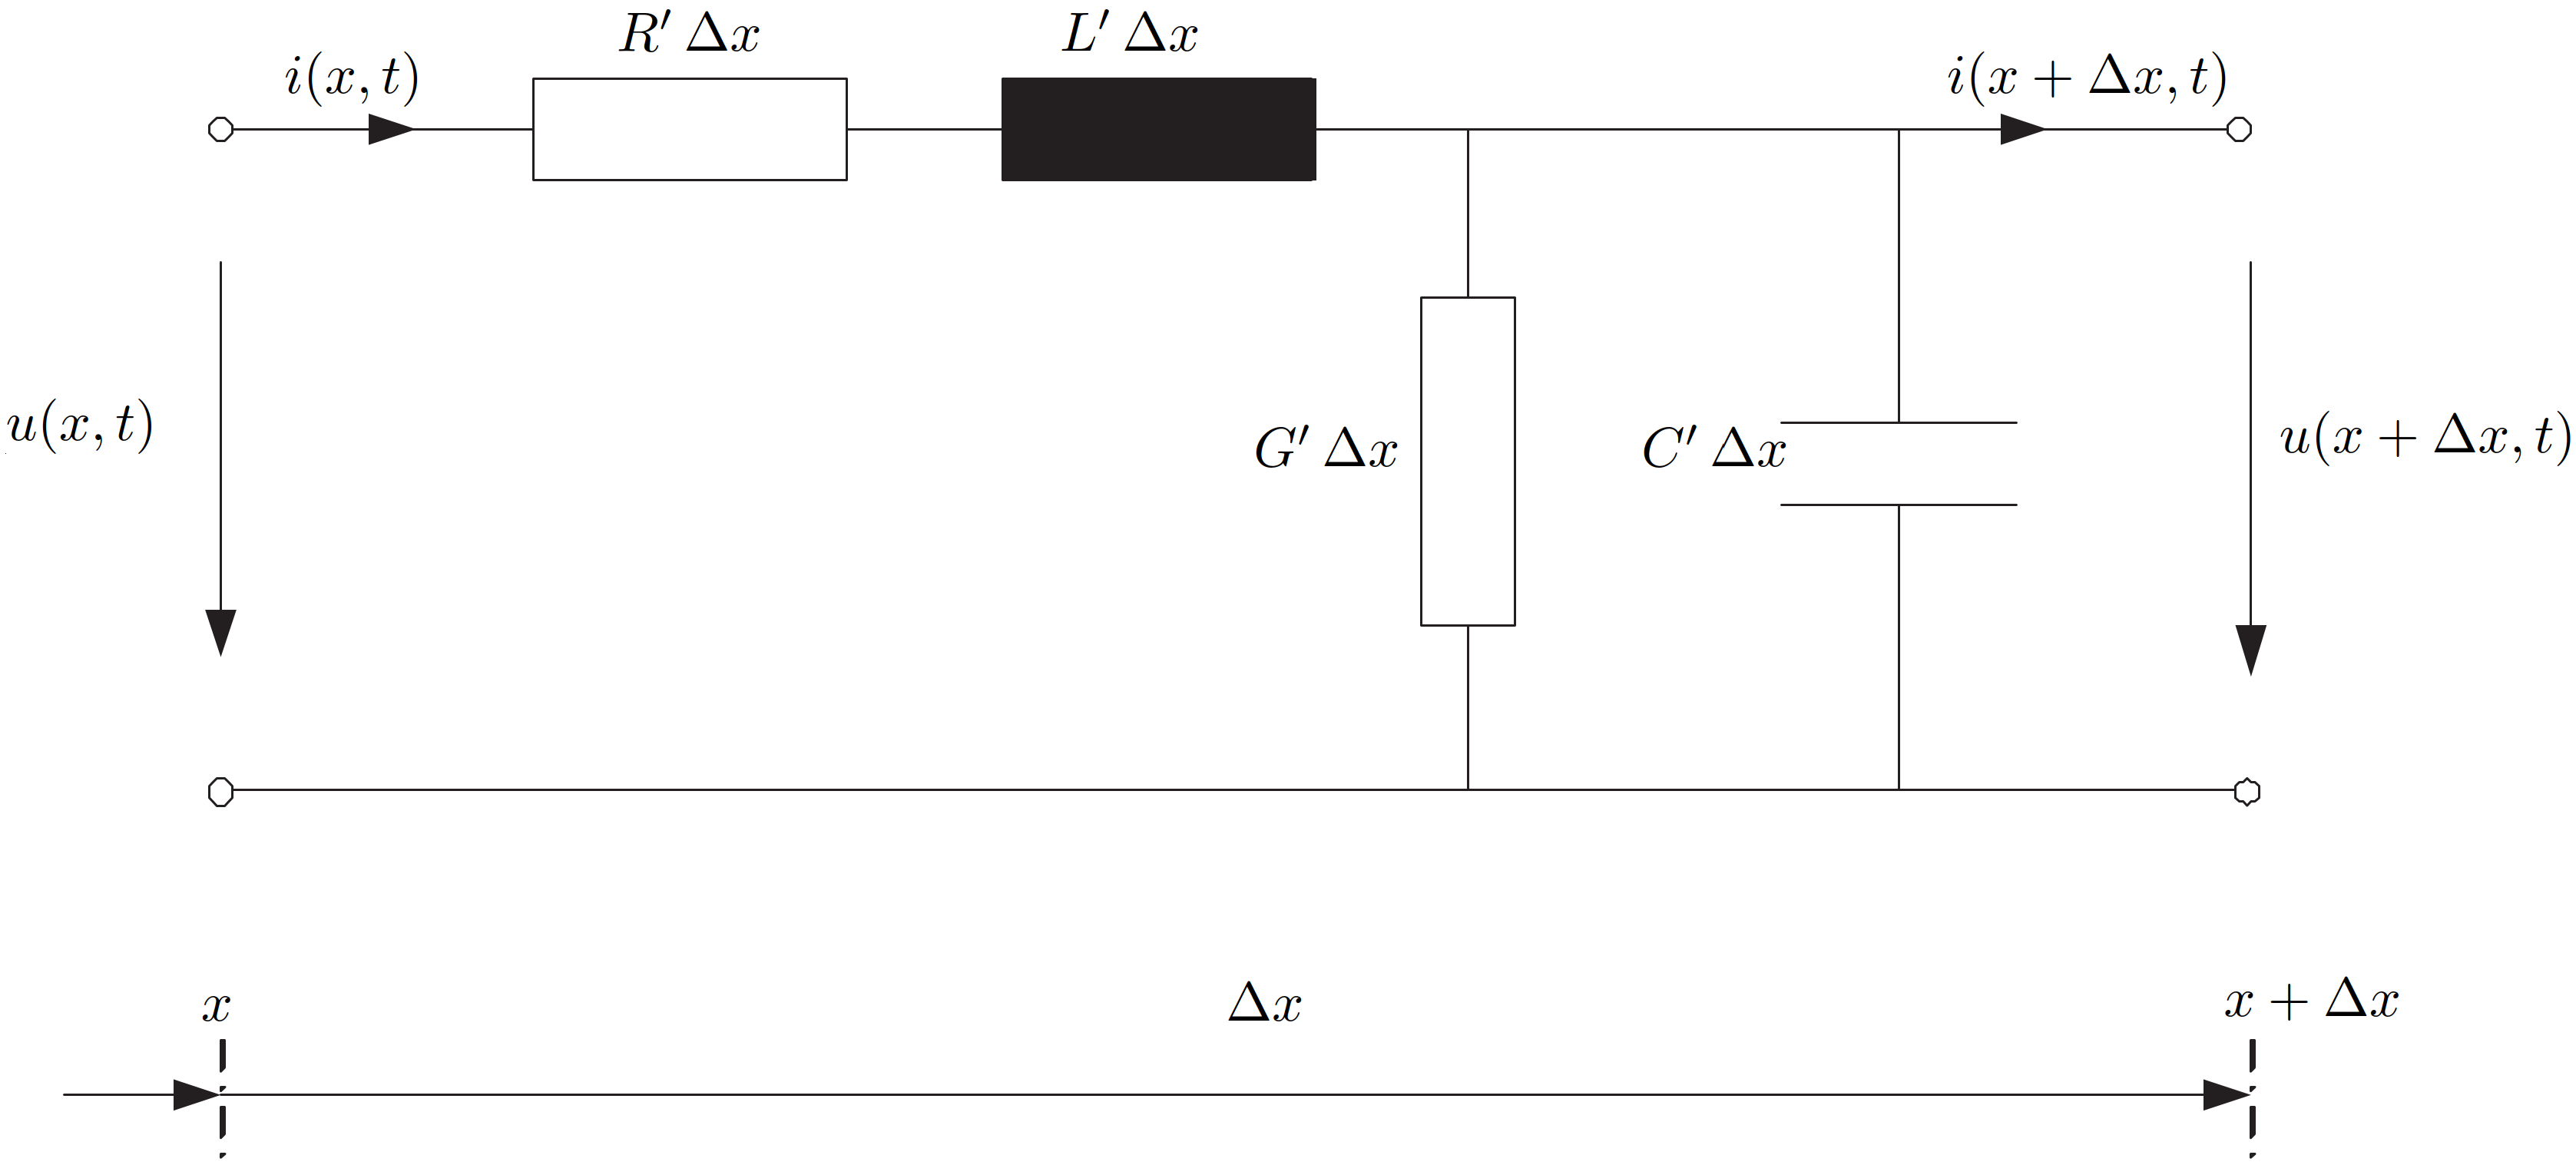
\includegraphics[width=0.98\columnwidth, align=c]{images/Leitungsgleichungen_1.png}

\vspace{0.15cm}

$\boxed{
\begin{pmatrix}
    \underline{U}_1 \\
    \underline{I}_1
    \end{pmatrix}
    =
    \begin{pmatrix}
    \cosh(\underline{\gamma} \cdot l) & Z_W \cdot \sinh(\underline{\gamma} \cdot l) \\
    \frac{1}{Z_W} \cdot \sinh(\underline{\gamma} \cdot l) & \cosh(\underline{\gamma} \cdot l)
    \end{pmatrix}
    \begin{pmatrix}
    U_2 \\
    \underline{I}_2
\end{pmatrix}}
$


\subsubsection{Modell Vereinfacht}

Wenn folgende 3 Punkte zutreffen, kann diese Vereinfachung angewendet werden:\\
\begin{itemize}
    \item $| \underline{\gamma } \cdot l | \ll 1$
    \item $\text{sinh}(\underline{\gamma } \cdot l) \approx \underline{\gamma } \cdot l$
    \item $\text{cosh}(\underline{\gamma } \cdot l) \approx 1$
\end{itemize}

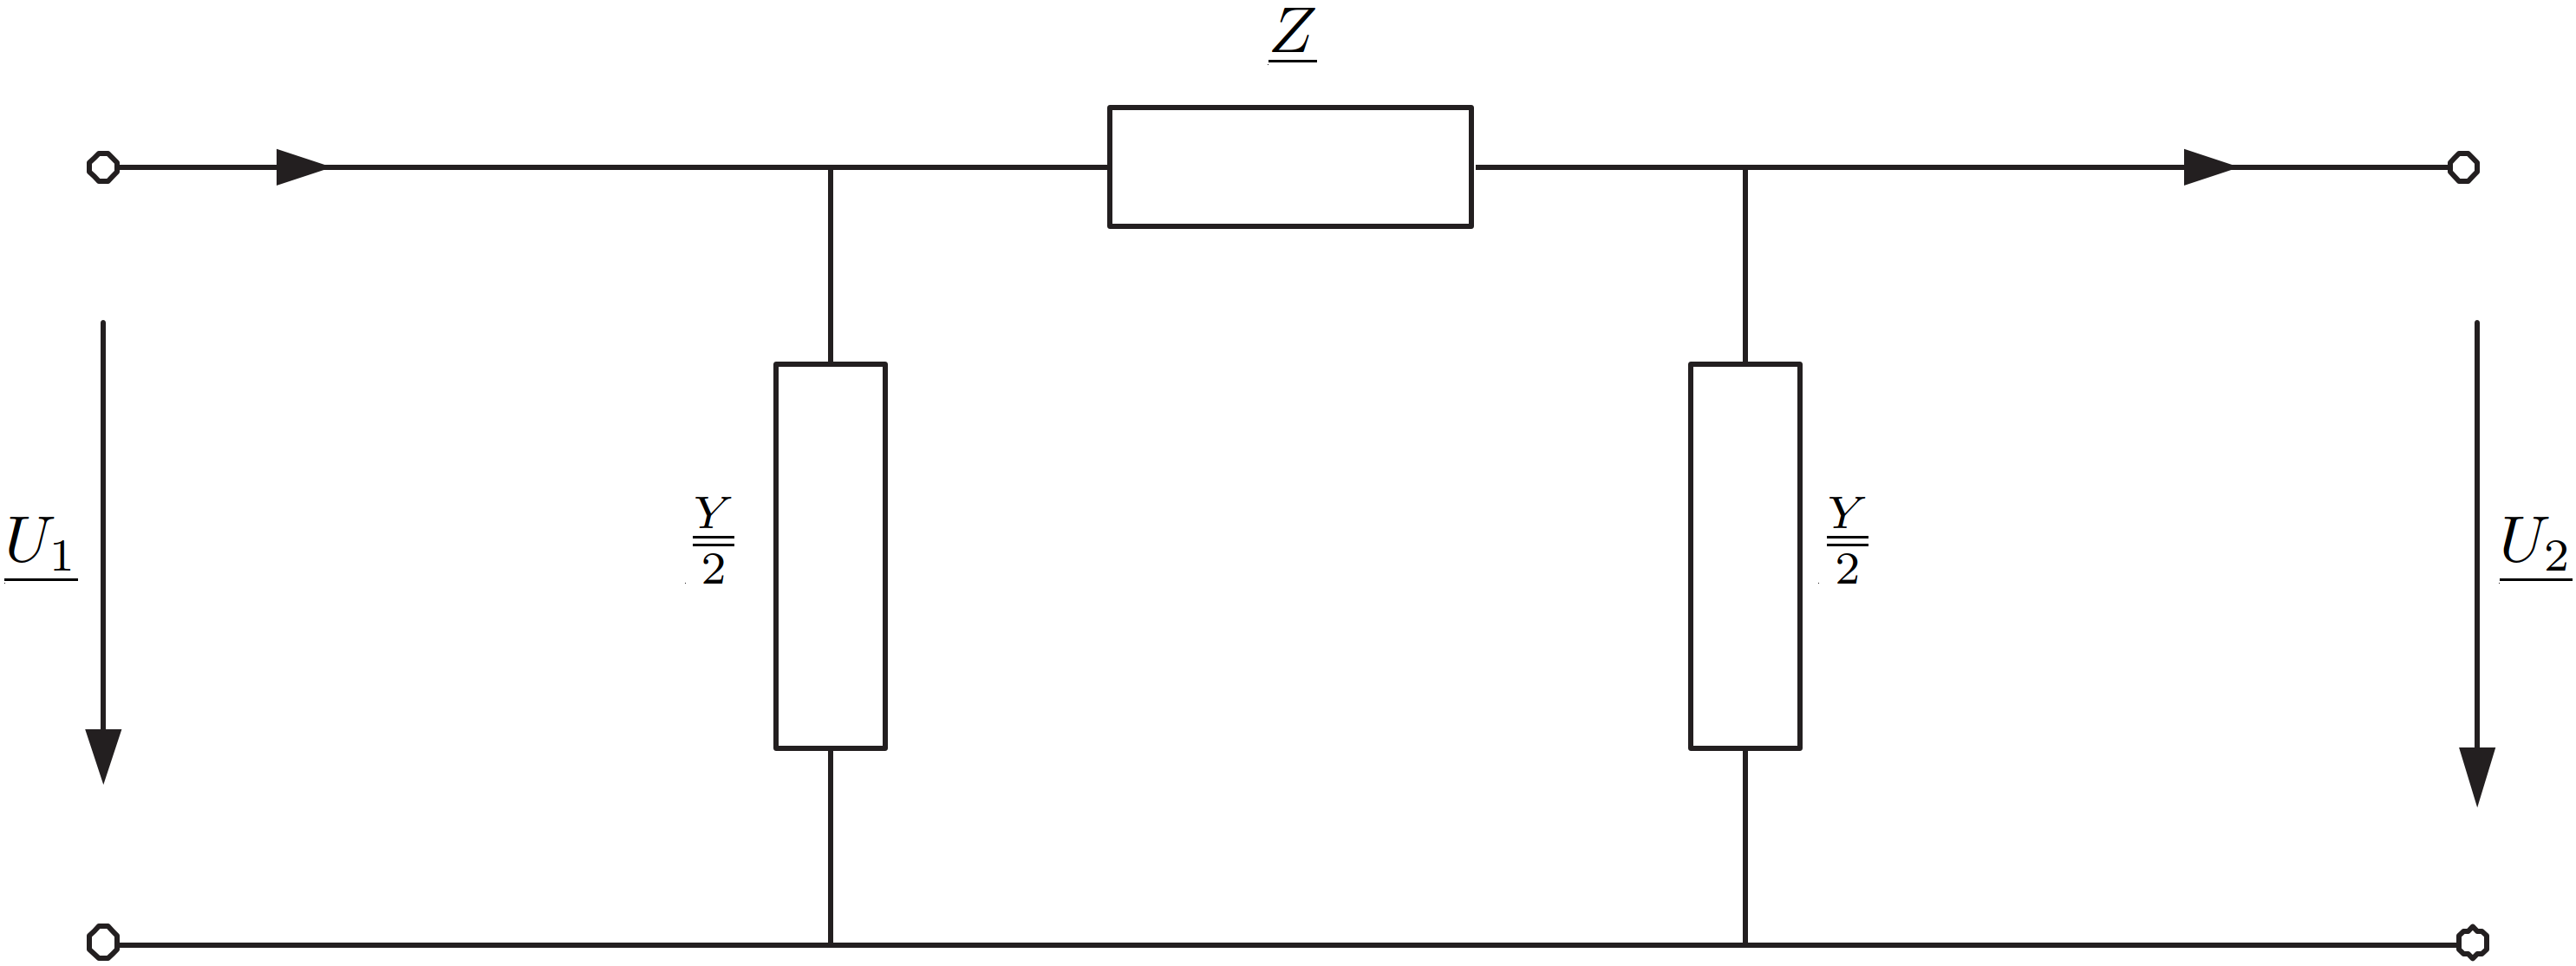
\includegraphics[width=0.98\columnwidth, align=c]{images/Leitungsgleichungen_2.png}

\vspace{0.15cm}

$\boxed{
\begin{pmatrix}
    \underline{U}_1 \\
    \underline{I}_1
    \end{pmatrix}
    =
    \begin{pmatrix}
    1 + \underline{Z} \cdot \dfrac{\underline{Y}}{2} & \underline{Z} \\
    \dfrac{\underline{Y}}{2} \cdot \left( 2 + \underline{Z} \cdot \dfrac{\underline{Y}}{2} \right) & 1 + \underline{Z} \cdot \dfrac{\underline{Y}}{2}
    \end{pmatrix}
    \begin{pmatrix}
    U_2 \\
    \underline{I}_2
\end{pmatrix}
}
$

\vspace{0.15cm}

$
\boxed{
    \underline{Z} = (R' + jX') \cdot l
}
\quad
\boxed{
    \dfrac{\underline{Y}}{2} = \dfrac{(G' + jB') \cdot l}{2}
}
$


\subsection{Vereinfachung für "kurze" Leitungen}

Vereinfachung für „kurze“ Leitungen mit konzentrierten Elementen R, G, L, C
\begin{itemize}
    \item 50-Hz-Freileitungen bis ca. 250 km
    \item 50-Hz-Kabel bis ca. 50 km
\end{itemize}

\vspace{0.15cm}

\includegraphics[width=0.98\columnwidth, align=c]{images/Leitungsmodell_gültigkeit.png}

\vspace{0.15cm}




























